\subsection{Ingame Spieler Interface}\label{subsec:spieler-interface}

Bei \textbf{Breaking Worse} handelt es sich um ein 2D-Spiel mit Draufsicht: \\
\begin{figure}[h]
    \centering
    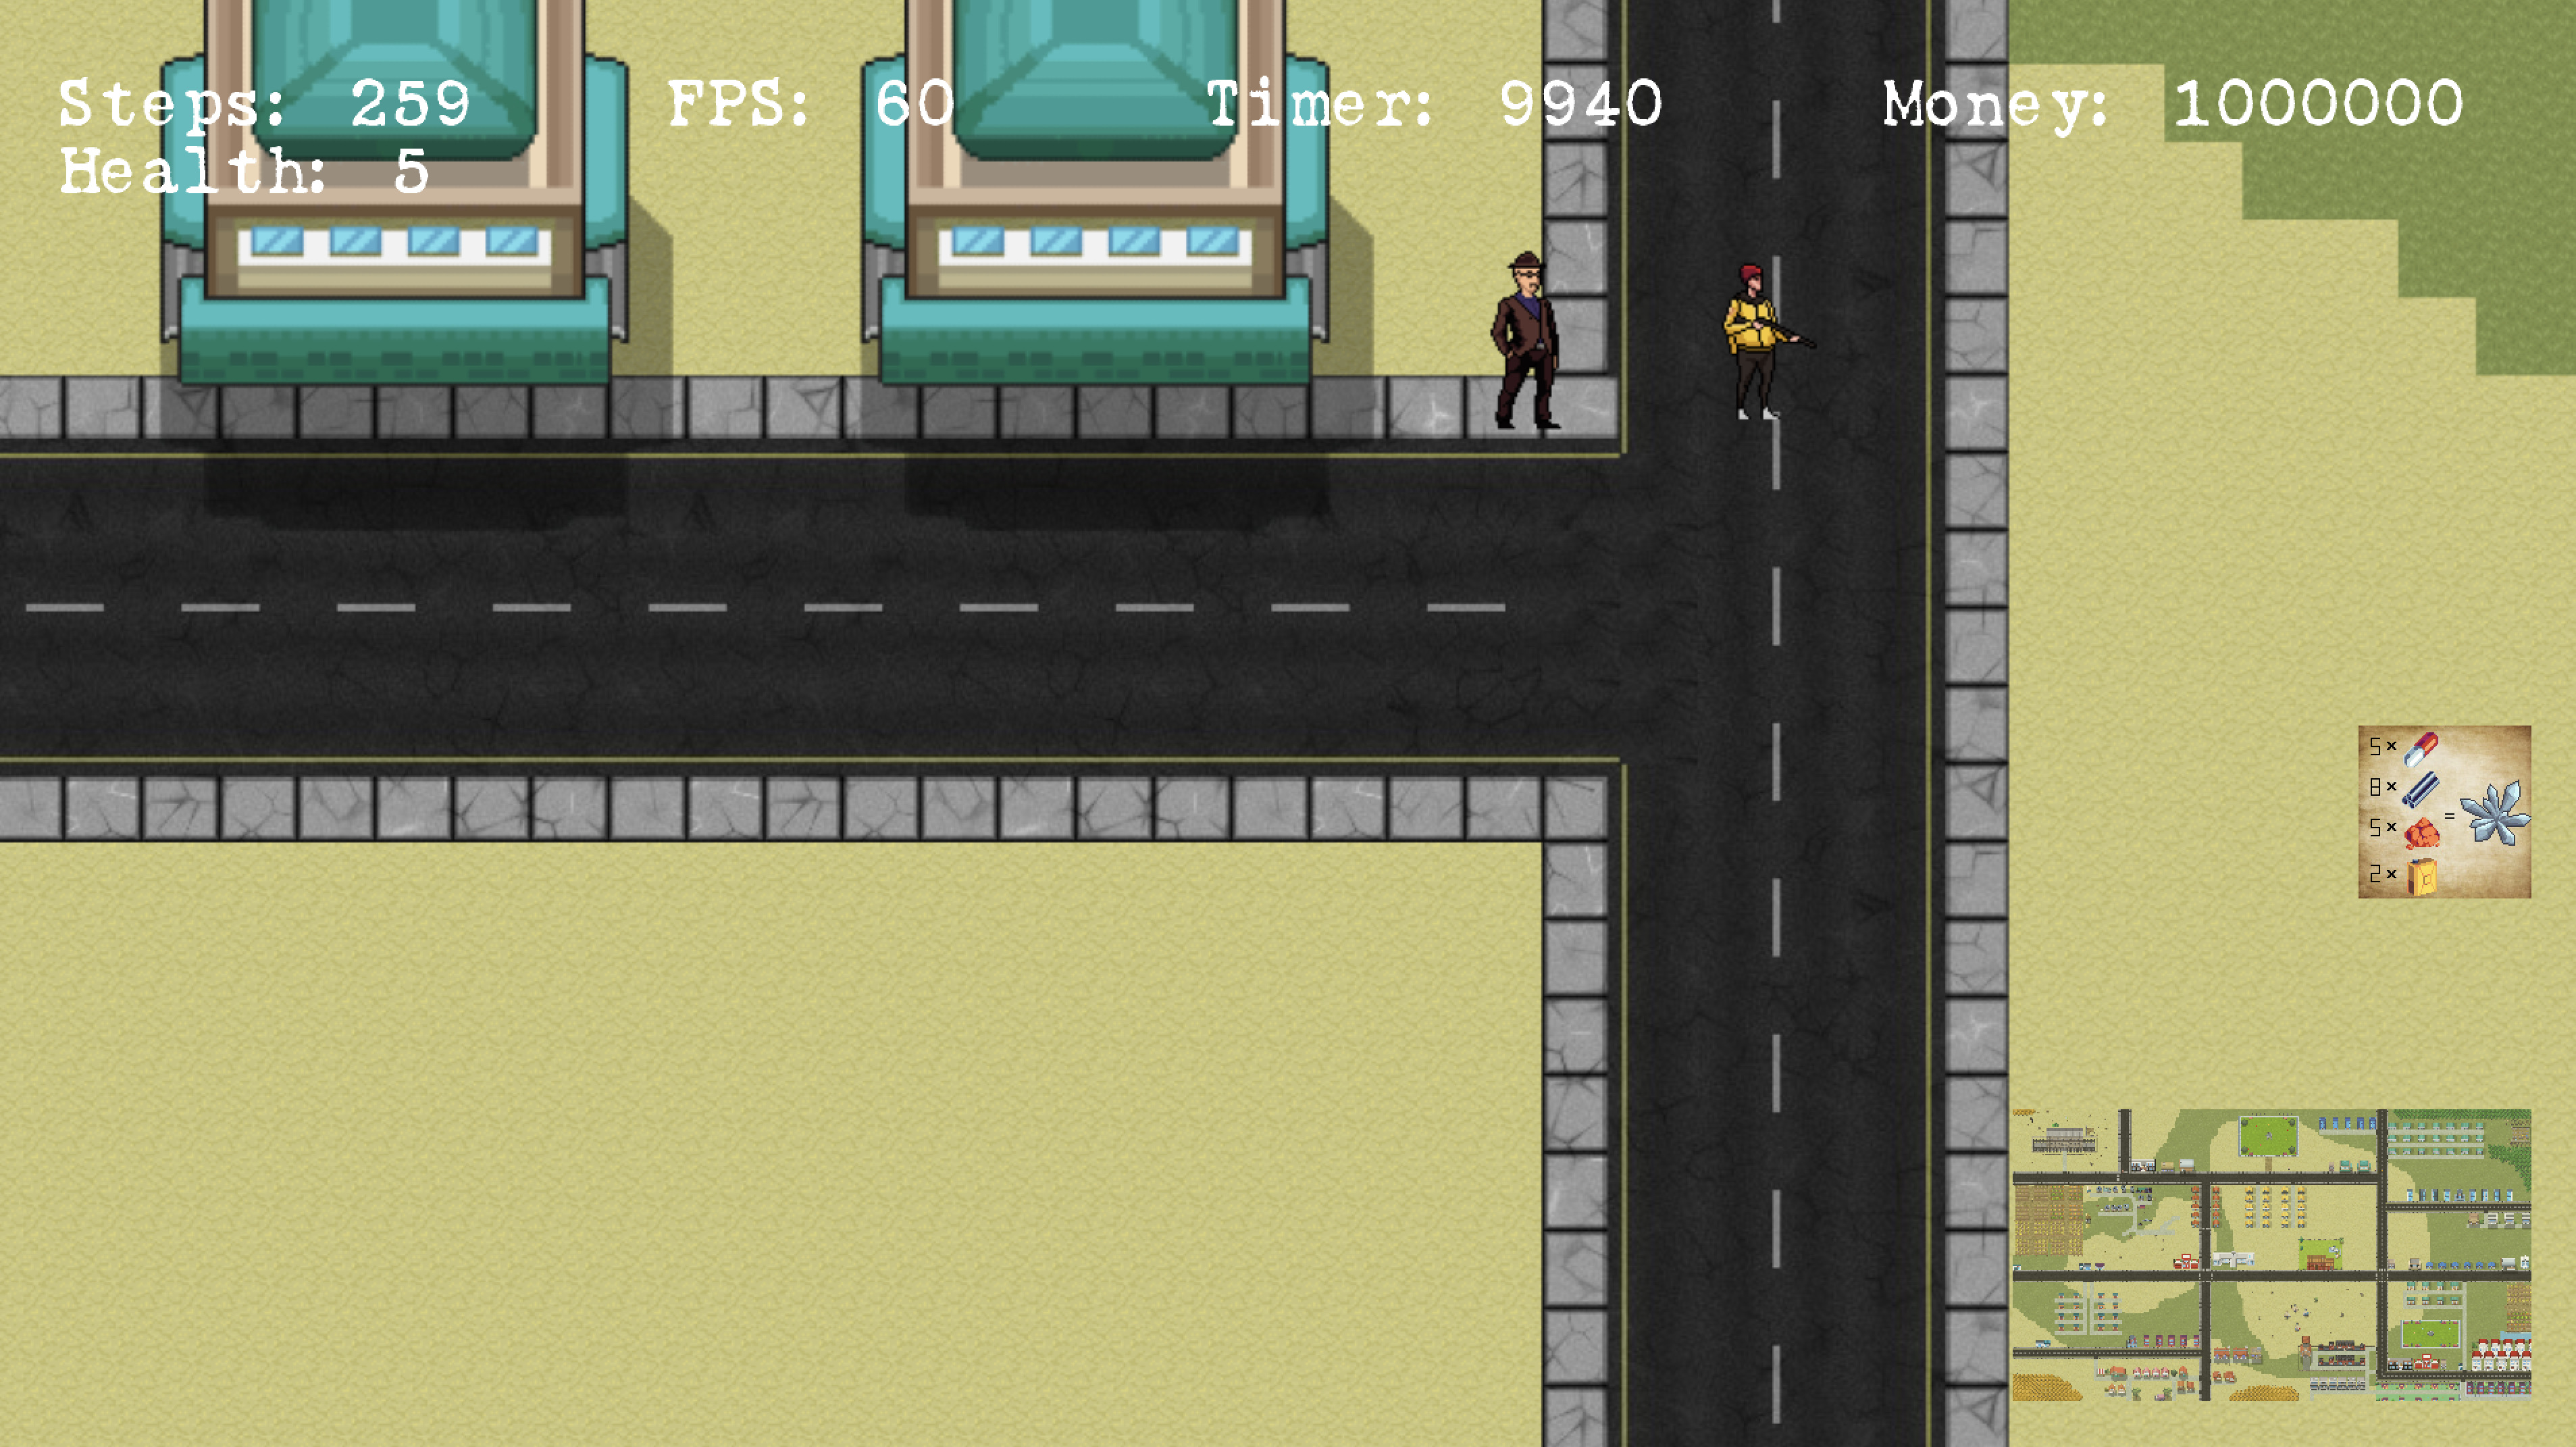
\includegraphics[width=0.85\textwidth]{./figures/InGameScreenBeispiel}
    \caption{Beispiel für Kameraperspektive mit HUD-Elementen (Farben und Icons werden noch angepasst)}
    \label{fig:figure}
\end{figure}\\
Dabei gibt es folgende HUD-Elemente:\\
\begin{itemize}
    \item \textbf{Minimap} \\
    Die Minimap ist ein von der Position der Spieler abhängiger Ausschnitt der Karte.
    Sie dient zur Orientierung und besseren Gefahren- und Fluchtwegerkennung der Spieler.
    \item \textbf{Wanted Status} \\
    Zeigt den Spielern an, wie aktiv die Polizei gerade nach ihnen fahndet.
    \item \textbf{Money} \\
    Zeigt den Spielern wie viel Geld sie gerade besitzen.
    \item \textbf{Timer} \\
    Zeigt den Spielern wie viel Zeit sie noch übrig haben bis der Todesfall durch die Krankheit eintritt.
    \item \textbf{Health Bar} \\
    Die Lebensleiste zeigt den Spielern wie viele Lebenspunkte sie gerade haben.
    \item \textbf{Zutatenliste} \\
    Die Zutatenliste zeigt den Spielern die nötigen Zutaten für das gerade ausgewählte Rezept an, sodass die Spieler sich nicht alle Zutaten auswendig merken müssen.
\end{itemize}


\subsubsection*{Steuerung}
Die zwei Spielcharaktere werden jeweils von einem Spielenden gesteuert.
Als Eingabegeräte wird das Benutzen zweier Controller (Playstation, XBox, etc.)
oder eines Controllers und einer Tastatur empfohlen.
Beide Spieler auf derselben Tastatur ist auch möglich, für die Standardbelegung
ist dafür jedoch ein Numpad erforderlich.
Sollte dieses nicht vorhanden sein, lässt sich die Steuerung beliebig anpassen. \\

\begin{table}[h!]
    \centering
    \begin{tabular}{|l|l|l|l|}
        \hline
        \multicolumn{2}{|c|}{\textbf{Tastatur}} & \textbf{Controller} & \textbf{Funktion} \\
        \hline
        \textbf{Spieler 1} & \textbf{Spieler 2} & & \\
        \hline
        W & Arrow-Up & Left-Joystick-Up & Bewegung nach oben \\&&& Menünavigation hoch \\
        \hline
        S & Arrow-Down & Left-Joystick-Down & Bewegung nach unten \\&&& Menünavigation runter \\
        \hline
        A & Arrow-Left & Left-Joystick-Left & Bewegung nach links \\
        \hline
        D & Arrow-Right & Left-Joystick-Right & Bewegung nach rechts \\
        \hline
        F & Numpad-2 & A / Cross & Interagieren \\
        \hline
        R & Numpad-3 & Y / Triangle & ausgerüstete Waffe wechseln \\
        \hline
        SPACE & Numpad-1 & X / Square & schlagen / schießen \\
        \hline
        TAB & Numpad-6 & Start / Options & Inventar öffnen \\
        \hline
        ESC & Numpad-9 & Back / Share & Pausenmenü öffnen \\
        \hline
    \end{tabular}
    \caption{Tastenbelegungen der vom Spieler ausführbaren Aktionen}
    \label{tab:steuerung}
\end{table}

\begin{description}
    \item[Bewegung]
    Mit den in \ref{tab:steuerung} beschrieben Tasten lässt sich der Spielcharakter bewegen. \\
    Bei Nutzung der Tastatur ist zusätzlich eine diagonale Bewegung möglich, indem zwei orthogonal
    zueinander gerichtete Bewegungen parallel ausgeführt werden. \\
    Bei Nutzung eines Controllers sind Bewegungen mit beliebiger Richtung möglich.
    \item[Interagieren]
    Mit der in \ref{tab:steuerung} definierten Taste lassen sich folgende Arten von
    Interaktionen durchführen:
    \begin{itemize}
        \item \textbf{Kochen}:
        Hierbei müssen sich beide Spielfiguren in der Nähe der CookingStation befinden
        und die in \ref{tab:steuerung} definierte Taste von einem der Spieler
        gedrückt werden.
        \item \textbf{Handeln}:
        Hierbei muss sich die Spielfigur in der Nähe eines interaktiven NPCs befinden.
        \item \textbf{Verstecken}:
        Hierbei muss sich die Spielfigur in der Nähe eines Busches befinden.
        \item \textbf{Türen durchschreiten}:
        Hierbei müssen sich beide Spielfiguren in der Nähe einer Tür befinden
        und die in \ref{tab:steuerung} definierte Taste von einem der Spieler
        gedrückt werden.
    \end{itemize}
    \item[ausgerüstete Waffe wechseln]
    Mit der in \ref{tab:steuerung} definierten Taste lässt sich zwischen Fäusten
    und Schusswaffe hin und her wechseln.
    \item[schlagen / schießen]
    Mit der in \ref{tab:steuerung} definierten Taste lässt sich die ausgerüstete Waffe
    anwenden, der Spielcharakter führt also einen Schlag bzw. einen Schuss aus.
    \item[Inventar öffnen]
    Mit der in \ref{tab:steuerung} definierten Taste lässt sich das Inventar-Fenster
    öffnen.
    \item[Pausenmenü]
    Mit der in \ref{tab:steuerung} definierten Taste lässt sich das Pausenmenü
    öffnen.
\end{description}
